% !TEX root=/home/tavant/these/manuscript/src/manuscript.tex


\section{Polytropic index in the \ac{HET} \ac{PIC} simulations}
\label{sec-PIC_poly}

We have developed in \cref{ch-3} a sheath model that uses a polytropic state law for the electrons instead of the usual isothermal approximation.
This model successfully reproduced the sheath characteristics  when no secondary electron emission where present (fully absorbing walls).
We now include the effects of the electron emission from the wall.

In this chapter, the \ac{PIC} simulations are the same as in \cref{sec-see}. 
Hence, the dielectric electrostatic boundary condition is not modeled, but instead the walls are grounded.
In addition, we recall that the axial convection is model using Lafleur's model of convection, as discussed in \cref{sec-reinjectionnoise}.

As previously done, we uses the mean values of the electron density $n_e$ and the electron pressure $ p_e = n_e T_e$ to find the value of the polytropic index.
\Cref{fig-radial_profiles_see} shows the radial profiles of the electron density and temperature for different values of the cross-over energy $\crover$.
The three values of $\crover$ are representative of the behaviour observed.
Indeed, $\crover=200\,\volt$ and $\crover=50\,\volt$ correspond to the upper and lower limits of regime {\bf II}, corresponding to low emission rate $\rate$, while regime {\bf I} corresponds to the case $\crover=10\,\volt$.
Regime {\bf II} is not presented has the oscillating nature of the sheath is not taken into account by the sheath modeled developed here. 


\begin{figure}[hbtp]
  \centering
  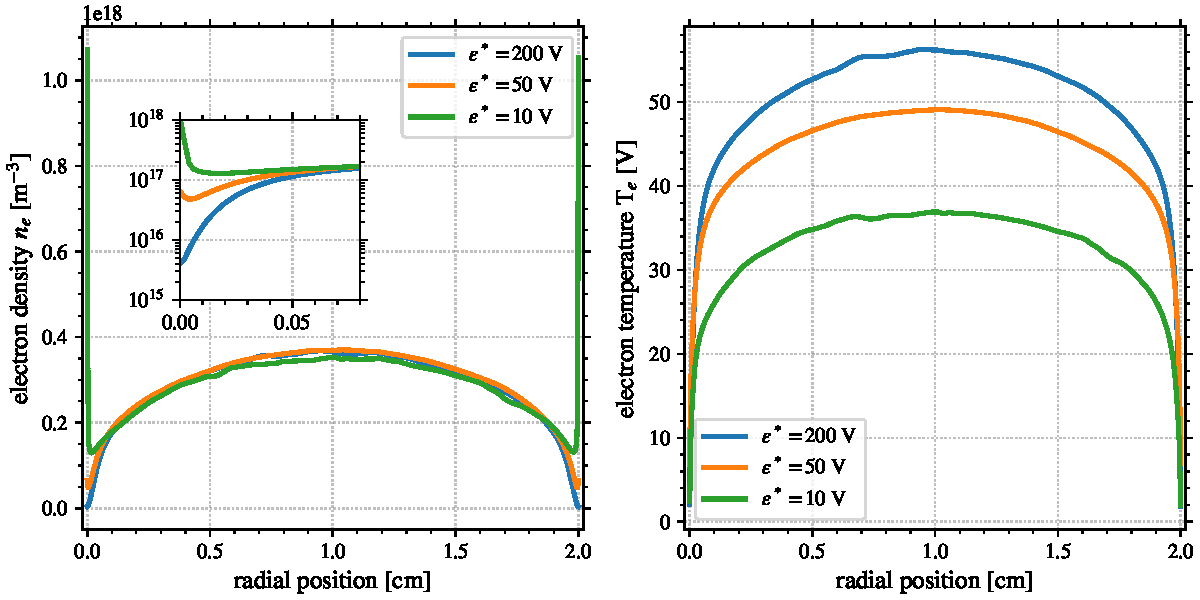
\includegraphics[width=\textwidth]{ne_Te_profiles.pdf}
  \caption{Radial profiles of (left) the electron density and (right) the electron temperature, for different values of $\crover$. The variables are averaged over the azimuthal direction and in time between $t=5\,\micro\second$ and $t=10\,\micro\second$.  }
  \label{fig-radial_profiles_see}
\end{figure}

We can see that the electron temperature presents a monotonic profile for all the values of $\crover$.
However, the electron density is not monotonic, but instead it presents an increase close to the wall.
This is clearly visible in \cref{fig-log_pe-ne} that presents the electron pressure as a function of the electron density, in log scale.
We see that close to the wall, where the electron pressure is the lowest, the curves present a significant inversion, in contrast with the case without electron emission seen in \cref{fig-polyFit}.
Otherwise in the rest of the domain, the curves are almost linear, corresponding to a polytropic low.

\begin{figure}[hbtp]
  \centering
  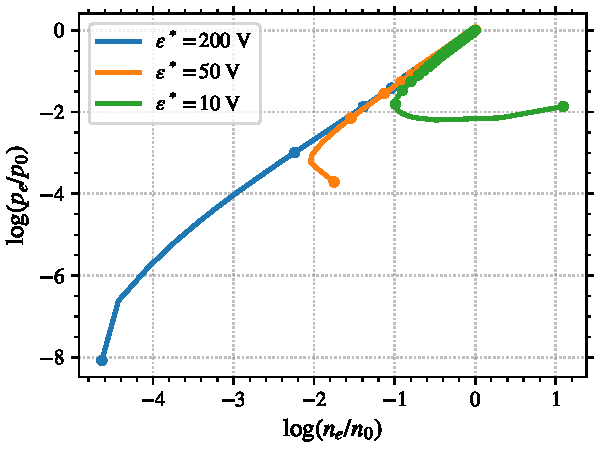
\includegraphics[width=\defaultwidth]{SEE_polytropic_presheath_and_sheath.pdf}
  \caption{Electron pressure as a function of the electron density normalized by the center variable, in log scale. The data corresponds to the same as \cref{fig-radial_profiles_see}. Markers are used every 10 cells ( corresponding to around one Debye length $\lde$)}
  \label{fig-log_pe-ne}
\end{figure}

\renewcommand\subfigurewidth{3in}

\begin{figure}[hbtp]
  \centering
  \begin{tabular}{c c}
    \subfigure{SEE_polytropic_presheath}{a}{20,20} & 
    \subfigure{SEE_polyfit}{a}{20,20} 
  \end{tabular}
  \caption{Polytropic fit for different values of $\crover$. The sheath (10 cells) are removed from the plots.}
  \label{fig-polyfit_see}
\end{figure}

% 
% \begin{figure}[hbtp]
%   \centering
%   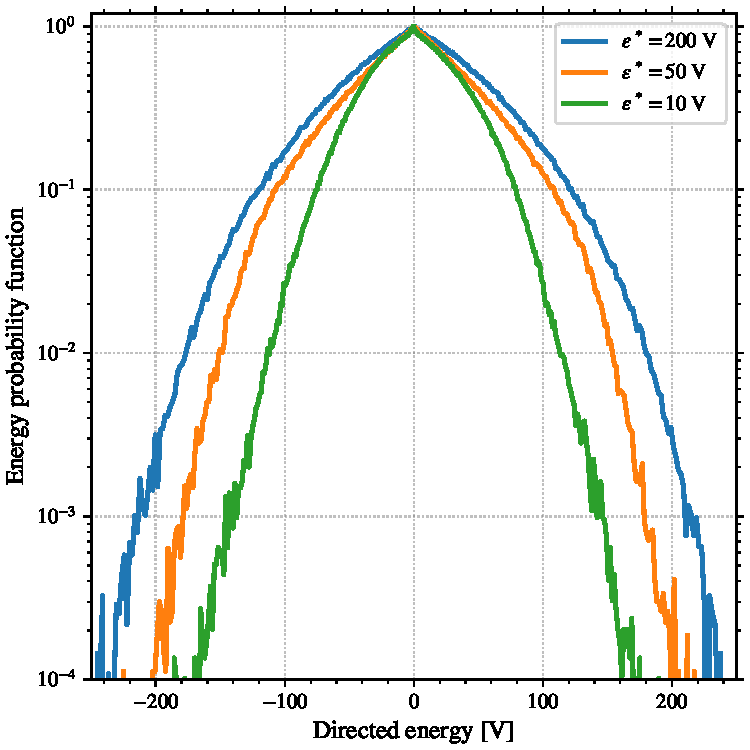
\includegraphics[width=\defaultwidth]{EVDF_Bulk.pdf}
%   \caption{Electron velocity distribution function at the center of the simulation, for different values of $\crover$.}
%   \label{fig-evdf_epsstar}
% \end{figure}


\FloatBarrier